% ICCIT 2026 submission. IEEE conference template, A4 (ICCIT requires the A4 template).
% DOUBLE-BLIND: no author names, affiliations, addresses, or emails anywhere.
% Every number here is verified in Defense/ICCIT/AUDIT_2026-08-21.md.
% Build: pdflatex main && bibtex main && pdflatex main && pdflatex main
\documentclass[conference,a4paper]{IEEEtran}
\IEEEoverridecommandlockouts
\usepackage{cite}
\usepackage{amsmath,amssymb,amsfonts}
\usepackage{graphicx}
\usepackage{textcomp}
\usepackage{xcolor}

\begin{document}

\title{MSA-YOLO: A Multi-Scale Attention Enhancement of YOLO for\\
Tiny-Human Detection in Aerial Search-and-Rescue Imagery}

% Double-blind submission: author block anonymized per ICCIT 2026 guidelines.
\author{\IEEEauthorblockN{Anonymous Submission}
\IEEEauthorblockA{\textit{Paper ID assigned by CMT}}}

\maketitle

\begin{abstract}
A person photographed from a drone over a disaster site may span fewer than ten
pixels, which is below the resolving limit of a standard detection head. This
paper presents MSA-YOLO, a multi-scale attention enhancement of YOLO11m for this
regime, and measures every component instead of assuming it helps. Two changes
define the detector: a convolutional block attention module replaces the
baseline self-attention block, and a stride-4 detection scale extends the head to
four levels. An additive ablation on the C2A disaster benchmark introduces one
change at a time. The stride-4 scale is the effective one, raising AP50 from
0.843 to 0.853 and recall of sub-8-pixel people from 0.743 to 0.757, while the
attention substitution removes about one million parameters and gives the lowest
latency of the four configurations. A bidirectional state-space neck, tested
under the same protocol, adds 2.4 million parameters and nearly triples latency
without improving any accuracy metric, and is reported as a negative result. A
tiny-aware change to label assignment then raises sub-8-pixel recall by a further
2.08 points with a bootstrap interval that excludes zero, replicated over three
training seeds. Finally, the detector is confronted with real footage collected
for this study. Zero-shot it reaches 0.335 AP50 on drone video and 0.133 on real
disaster frames; after fine-tuning with 248 labeled real frames it reaches 0.795
and 0.411 while the synthetic benchmark holds at 0.837. The recommended model
uses 19.6 million parameters and runs at 14.6 ms per image.
\end{abstract}

\begin{IEEEkeywords}
tiny object detection, aerial human detection, search and rescue, attention,
multi-scale detection, label assignment, UAV imagery
\end{IEEEkeywords}

\section{Introduction}
When an earthquake or a flood strikes, the first hours decide how many people
are found alive. A drone can sweep a disaster site far faster than a ground
team, but the imagery it returns is punishing to search by eye. A person seen
from altitude spans a few dozen pixels at best, and one sortie produces
thousands of frames. Automating that search is a practical need rather than a
convenience.

The difficulty is geometric. A one-stage detector predicts boxes on a grid whose
cell covers a stride-sized region of the input, so the finest standard scale, at
stride 8, summarizes an 8 by 8 pixel patch in one cell. A twelve-pixel person
spans about one and a half cells there and only a fraction of a cell at coarser
scales, and a detector cannot localize what falls inside a fraction of one cell.
In the C2A disaster benchmark used here~\cite{nihal2024c2a}, about 47\% of
annotated people are smaller than ten pixels. Remedies exist. Higher-resolution
detection scales~\cite{zhu2021tphyolov5}, feature
attention~\cite{woo2018cbam,wang2020eca}, sliced
inference~\cite{akyon2022sahi} and, more recently, state-space
necks~\cite{gu2023mamba,wang2025mambayolo} have all been proposed, but they are
usually reported one at a time, on generic aerial data, and without a shared
training protocol. Anyone building a deployable rescue detector today has to
guess which addition earns its cost.

This paper replaces that guess with a measurement, and then pushes past the
benchmark. We present MSA-YOLO, which modifies YOLO11m~\cite{jocher2024yolo11}
in exactly two places, and evaluate it through an additive ablation in which one
component is introduced at a time under an identical protocol. We then show that
the remaining error at the smallest sizes is better attacked in the label
assigner than in the network, and finally we test the detector on real drone and
disaster footage that we collected and annotated, because a model trained on
composited scenes has never been asked what it does on real ones.

The contributions are the following.
\begin{itemize}
\item MSA-YOLO, an attention-and-scale enhancement of YOLO11m whose components
are attributed individually: the stride-4 scale raises AP50 from 0.843 to 0.853
and sub-8-pixel recall from 0.743 to 0.757, and the attention substitution
arrives at a negative parameter cost. The recommended configuration is second
only to a detector three times its size among published results on C2A.
\item A documented negative result for a bidirectional state-space neck, which
costs 2.4 million parameters and 2.8 times the latency for no accuracy gain.
\item A tiny-aware label-assignment blend that adds 2.08 points of sub-8-pixel
recall at no parameter or inference cost, with a bootstrap confidence interval
that excludes zero and a positive effect in all three training seeds tested.
\item A real-footage study on our own drone, campus and disaster imagery that
quantifies the synthetic-to-real gap, shows what 248 labeled frames buy, and
reports where that budget stops paying.
\end{itemize}

\section{Related Work}
Object detection divides into two-stage detectors in the R-CNN
line~\cite{ren2015fasterrcnn,cai2018cascade}, one-stage detectors such as
SSD~\cite{liu2016ssd}, RetinaNet~\cite{lin2017focal} and the YOLO
family~\cite{redmon2016yolo,wang2024yolov9,jocher2024yolo11}, and
transformer designs such as DETR~\cite{carion2020detr} and
RT-DETR~\cite{zhao2024rtdetr}. We work inside the one-stage YOLO family because
its speed and small model size suit airborne deployment.

Detecting very small objects is a distinct problem~\cite{cheng2023smallobject}.
Three lines of work address it: adding higher-resolution detection scales, where
feature pyramids~\cite{lin2017fpn} and a stride-4 head extend detection to
targets a few pixels wide~\cite{zhu2021tphyolov5}; re-weighting features with
attention, where channel attention~\cite{wang2020eca} and combined
channel-and-spatial attention~\cite{woo2018cbam} are the common choices; and
operating at inference time, where slicing runs the detector over overlapping
crops~\cite{akyon2022sahi}. A fourth line changes neither the network nor the
input but the training step that selects positive samples. Its observation is
that intersection over union collapses for tiny boxes, so
Wang et al.~\cite{wang2021nwd} replaced it with a normalized Wasserstein
distance, RFLA~\cite{xu2022rfla} built an assignment strategy on a
receptive-field prior, and SimD~\cite{shi2024simd} learned an adaptive
similarity. Modern YOLO versions assign samples with the task-aligned assigner
of TOOD~\cite{feng2021tood}, which still scores localization with the IoU
family, and none of the tiny-object assignment work above has been applied
inside it for aerial person detection. Section~\ref{sec:assign} takes that
opening.

For data, real search-and-rescue collections such as
SARD~\cite{sambolek2021sard} and HERIDAL~\cite{bozic2019heridal} hold only a few
thousand frames. C2A~\cite{nihal2024c2a} instead composites segmented human
figures onto real disaster backgrounds~\cite{kyrkou2020aider}, giving 10{,}215
images and roughly 360{,}000 instances. Results on such data are almost always
in-domain, which leaves transfer untested. Work on domain
randomization~\cite{tobin2017domainrand} and on fine-tuning synthetic-trained
models with a little real data~\cite{tremblay2018synthetic} suggests the recipe
we follow in Section~\ref{sec:real}.

\section{MSA-YOLO}

\subsection{Overall Architecture}
The pipeline is shown in Fig.~\ref{fig:arch}. An aerial image is
letterbox-resized to $640 \times 640$ and passed through the YOLO11m backbone,
in which the terminal self-attention block is replaced by a convolutional block
attention module. The path-aggregation neck then fuses features across scales,
carrying the top-down pass one level further than the standard design so that a
stride-4 branch is produced, and a four-scale head decodes boxes before
non-maximum suppression. Only these two elements differ from the baseline, which
is what allows the ablation of Section~\ref{sec:ablation} to attribute each
measured change.

\begin{figure*}[t]
\centerline{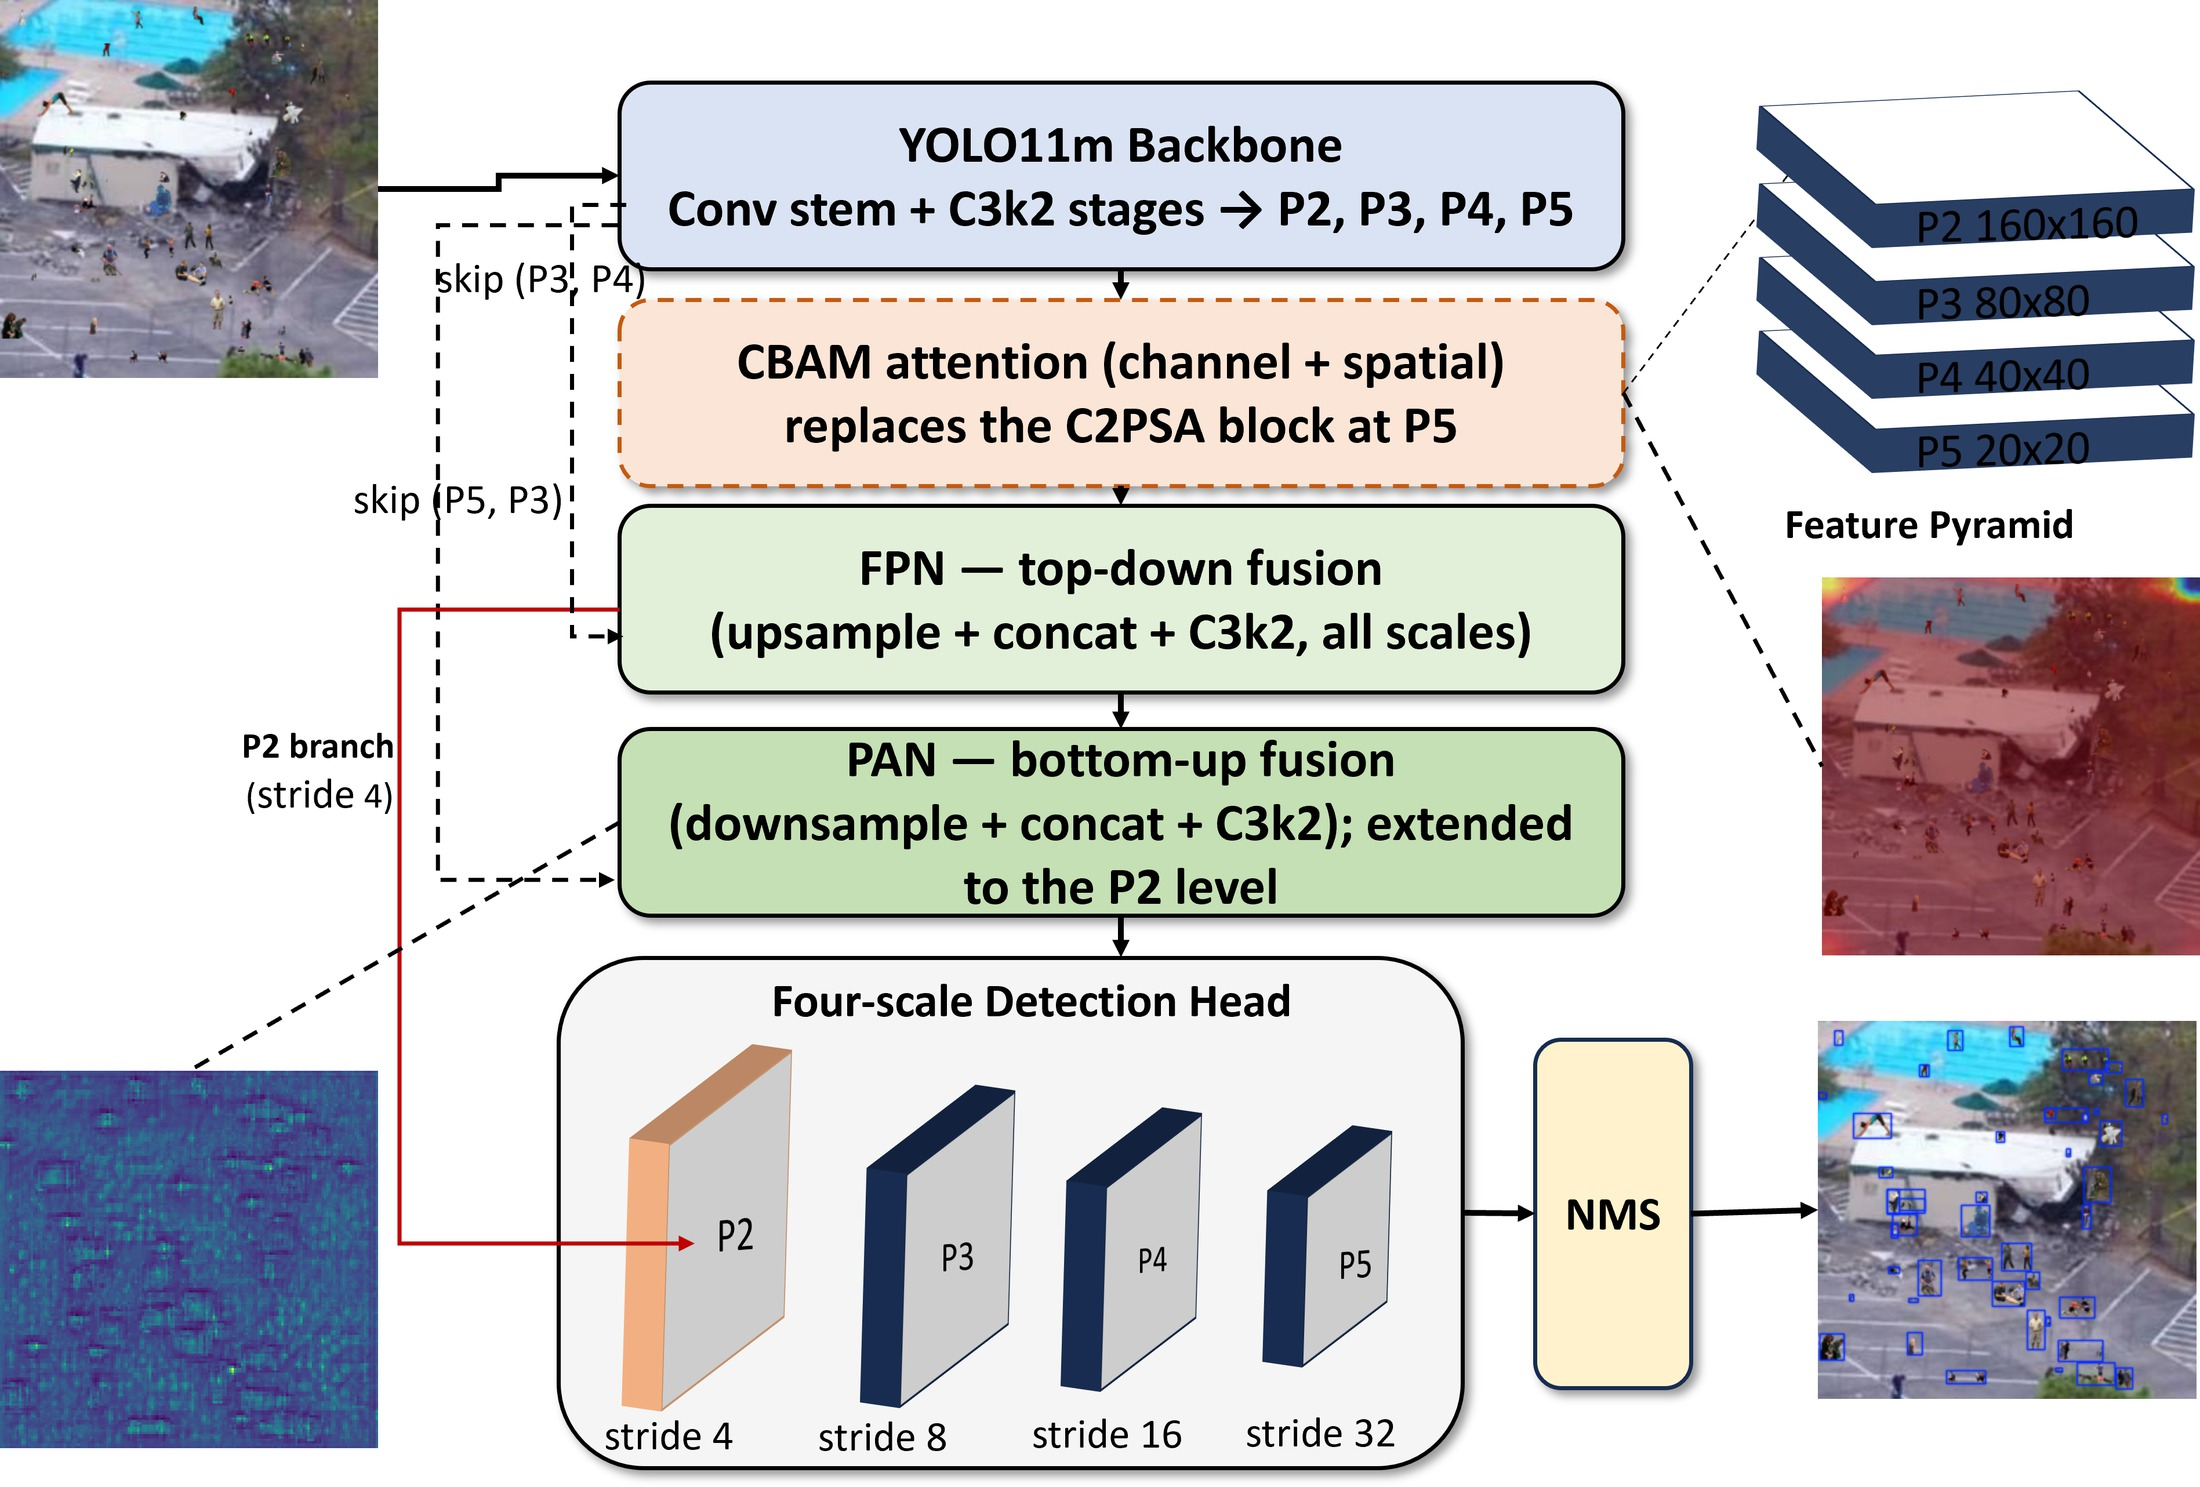
\includegraphics[width=0.94\textwidth]{figures/fig_arch.jpg}}
\caption{MSA-YOLO on a C2A scene. The backbone produces features at five
resolutions; CBAM (orange) replaces the terminal self-attention block and
re-weights the deepest features; the neck fuses scales and is carried one level
further than the standard design to produce a stride-4 branch, so the head
decodes at strides 4, 8, 16 and 32. The insets are the model's own signals on
this scene: input, attention response, stride-4 feature response, and final
detections. Note that the stride-4 map responds at the smallest scattered
figures, which the stride-8 level summarizes into single cells.}
\label{fig:arch}
\end{figure*}

\subsection{Attention Substitution}
The baseline places a self-attention block after the spatial-pyramid-pooling
stage. MSA-YOLO replaces it with a convolutional block attention
module~\cite{woo2018cbam}, which applies channel attention followed by spatial
attention. For a feature map $\mathbf{F} \in \mathbb{R}^{C \times H \times W}$,
\begin{align}
  \mathbf{M}_c(\mathbf{F}) &= \sigma\big(\mathrm{MLP}(\mathrm{AvgPool}(\mathbf{F}))
      + \mathrm{MLP}(\mathrm{MaxPool}(\mathbf{F}))\big), \\
  \mathbf{M}_s(\mathbf{F}') &= \sigma\big(f^{7\times7}([\mathrm{AvgPool}(\mathbf{F}');
      \mathrm{MaxPool}(\mathbf{F}')])\big),
\end{align}
where $\sigma$ is the sigmoid function and $f^{7\times7}$ a convolution with a
$7\times7$ kernel, and the map is refined as
$\mathbf{F}' = \mathbf{M}_c(\mathbf{F}) \otimes \mathbf{F}$ then
$\mathbf{F}'' = \mathbf{M}_s(\mathbf{F}') \otimes \mathbf{F}'$. The module uses a
reduction ratio of 16. Because it is lighter than the block it replaces, the
substitution lowers the parameter count relative to the baseline, so any gain it
brings is obtained at negative parameter cost.

\subsection{The Stride-4 Detection Scale}
A detection cell summarizes a stride-sized region, so a target of side $s$
pixels spans $s/d$ cells at stride $d$. At stride 8 a twelve-pixel person covers
about 1.5 cells; at stride 4 it covers about three, which is the first level
offering enough spatial support to localize it. MSA-YOLO therefore continues the
neck's top-down pass one level below the standard design: the fused stride-8
feature is upsampled, concatenated with the high-resolution backbone feature at
stride 4, and fused into a $160 \times 160$ map that a fourth detection branch
reads. The existing three levels are untouched, which keeps the addition
attributable.

\subsection{Tiny-Aware Label Assignment}
\label{sec:assign}
The changes above alter the network. The remaining error at the smallest sizes,
however, is partly created during training. Modern YOLO versions select positive
samples with a task-aligned assigner that scores each candidate by
$t = s^{p} u^{q}$, where $s$ is a classification score and $u$ a localization
overlap measured with the complete IoU. That measurement is the weak point at
this scale: for a person a few pixels wide, a one-pixel offset can drive the IoU
to zero, so candidates for the smallest targets are ranked with almost no signal
and those people are trained on poorly chosen samples.

We keep the assigner and replace only its overlap term. For a ground-truth box
$g$ and a candidate $b$ with centers, widths and heights $(c_x, c_y, w, h)$, the
squared 2-Wasserstein distance between Gaussians fitted to the boxes is
\begin{equation}
  W_2^2(g,b) = (c_{x}^{g}\!-\!c_{x}^{b})^2 + (c_{y}^{g}\!-\!c_{y}^{b})^2
    + \tfrac{1}{4}\big[(w^{g}\!-\!w^{b})^2 + (h^{g}\!-\!h^{b})^2\big],
\end{equation}
and the normalized Wasserstein similarity~\cite{wang2021nwd} maps it into
$(0,1]$ as $S(g,b) = \exp(-W_2(g,b)/C)$ with $C$ set to the median person size
of the dataset in pixels, here 12.8. Unlike the IoU, this similarity stays
informative for disjoint tiny boxes: a near miss scores above a distant one even
when both overlap nothing. The overlap the assigner consumes becomes
\begin{equation}
  u = (1-\gamma)\,\mathrm{CIoU}(g,b) + \gamma\, S(g,b),
  \label{eq:blend}
\end{equation}
where $\gamma$ sets how far assignment trusts the scale-robust similarity, and
$\gamma = 0$ recovers the unmodified assigner. The change affects training only.
It adds no parameters and no inference cost, and it is distinct from placing the
same distance inside the regression loss, which we also tried without success.

\subsection{An Explored State-Space Neck}
To test the claim that state-space blocks improve feature aggregation, a variant
replaces the bottleneck at six neck layers with a block performing bidirectional
local-window selective scans, inserted so that the backbone and the head are
unchanged. Its scan diagnostics confirm the module was active, with a mean
forward-to-reverse cosine distance of 0.836. Section~\ref{sec:ablation} reports
what it cost and what it bought.

\section{Experimental Setup}
All training and evaluation ran on one workstation with an NVIDIA RTX 4070 Ti
SUPER (16 GB), an Intel Core i7-14700K and 128 GB of RAM, using Python 3.11,
PyTorch 2.12 with CUDA 12.6, and Ultralytics 8.4.56. Every configuration used
AdamW at a base learning rate of 0.001 with a cosine schedule, up to 300 epochs
with early stopping on fitness and on $F_2$, mixed precision, and seed 0. The
optimizer was pinned because the framework default diverged on the four-scale
head. Batch size was 16, reduced to 8 physical with gradient accumulation for
the stride-4 models, whose extra scale raises activation memory.

C2A~\cite{nihal2024c2a} provides 10{,}215 images with roughly 360{,}000 person
instances across collapsed-building, fire, flood and traffic scenes. Two
protocols are used, and they are never mixed within a table. The
\emph{official} split (6{,}129 training, 2{,}043 validation, 2{,}043 test
images) carries the ablation of Section~\ref{sec:ablation}, because published
results on this benchmark use it. An audit of scene identifiers, however, found
that 98\% of official test scenes also appear in training, since several
composited images share one background. We therefore also built a
\emph{scene-disjoint} re-split (6{,}135 / 2{,}040 / 2{,}040) in which all images
of a scene fall on one side. Retraining the recommended model there costs 1.6
points of AP50 and 1.2 points of sub-8-pixel recall, so the leakage inflates the
official protocol modestly and changes no conclusion. All assignment and
real-footage experiments use the clean split.

Because a missed person costs more than a false alarm, the primary operating
metric is the recall-weighted $F_2$ score. We also report AP50, COCO average
precision, average recall at 100 detections, recall in the size bands very-tiny
(under 8 px), tiny (8 to 16 px), small (16 to 32 px) and medium (32 to 96 px)
measured as the square root of box area, and end-to-end latency including
preprocessing and non-maximum suppression. Where two models are compared on one
set, a paired image-level bootstrap over 1{,}000 resamples gives a 95\%
confidence interval and a two-sided $p$-value.

\section{Results}
\label{sec:ablation}

\subsection{Additive Ablation}
Table~\ref{tab:abl} reports the four configurations on the official C2A test
set. Aggregate average precision is saturated, with all four models inside 0.002
AP of one another, which is expected when annotation noise dominates at strict
IoU thresholds for boxes this small. The differences appear where the task
lives. The stride-4 scale is the effective change: it lifts AP50 from 0.843 to
0.853, average recall from 0.691 to 0.703, sub-8-pixel recall from 0.743 to
0.757, and operational $F_2$ from 0.840 to 0.844, for about half a million
parameters and one millisecond. The attention substitution is close to free. It
removes roughly one million parameters relative to the baseline, gives the
lowest latency of the four, and improves every accuracy column slightly. The
state-space neck is the outlier in the wrong direction, adding 2.4 million
parameters and taking latency from 14.6 to 41.1 ms while matching, not beating,
the configuration below it. On this evidence MSA-YOLO is the attention plus
stride-4 configuration, and the state-space neck is not carried forward.

\begin{table}[htbp]
\caption{Additive Ablation on the Official C2A Test Split. Par.\ is parameters
in millions, GF is GFLOPs, AR is average recall at 100 detections, VT is recall
below 8 px, and ms is end-to-end latency. The last row adds the state-space
neck on top of CBAM and P2.}
\label{tab:abl}
\begin{center}
\footnotesize
\setlength{\tabcolsep}{3pt}
\begin{tabular}{|l|c|c|c|c|c|c|c|}
\hline
\textbf{Configuration} & \textbf{Par.} & \textbf{GF} & \textbf{AP50} & \textbf{AP} & \textbf{AR} & \textbf{VT} & \textbf{ms} \\
\hline
YOLO11m & 20.03 & 67.7 & 0.843 & 0.615 & 0.691 & 0.743 & 13.7 \\
\hline
+ CBAM & 19.08 & 66.9 & 0.847 & 0.616 & 0.692 & 0.746 & 13.5 \\
\hline
+ CBAM + P2 & 19.57 & 86.7 & \textbf{0.853} & 0.615 & 0.703 & \textbf{0.757} & 14.6 \\
\hline
+ SSM neck & 22.01 & 98.4 & 0.852 & 0.614 & 0.704 & 0.757 & 41.1 \\
\hline
\end{tabular}
\end{center}
\end{table}

Recall by size explains the flat aggregate. The stride-4 scale trades a little
accuracy on larger targets for its gain at the bottom: tiny-band recall moves
from 0.869 to 0.865 and small-band recall from 0.894 to 0.886, while the medium
band falls from 0.909 to 0.808. That last figure looks severe but rests on only
317 of roughly 72{,}500 test instances, so it is noisy. The net effect is a
model that is better where the dataset actually lives, since 99.6\% of instances
are below 32 px. Calibration is stable across the chain, with expected
calibration error between 0.020 and 0.023, so a reported confidence can be read
as an empirical precision.

\subsection{Comparison with Published Detectors}
Table~\ref{tab:sota} places MSA-YOLO against the results reported by Nihal et
al.~\cite{nihal2024c2a} on the same test split, none of which use slicing or
test-time augmentation. MSA-YOLO exceeds every convolutional and transformer
baseline in that study except YOLOv9-e, and it does so with 19.6 million
parameters against that model's 57.3 million. For a detector that must ride on
airborne hardware, giving up four points of AP50 for a third of the size is the
trade worth making.

\begin{table}[htbp]
\caption{Comparison with Published Results on C2A. The upper block is as
reported by Nihal et al.~\cite{nihal2024c2a} on the same test split; no entry
uses slicing or test-time augmentation.}
\label{tab:sota}
\begin{center}
\small
\begin{tabular}{|l|c|c|c|}
\hline
\textbf{Model} & \textbf{AP50} & \textbf{AP} & \textbf{Params} \\
\hline
Faster R-CNN & 0.634 & 0.366 & $\sim$41M \\
\hline
RetinaNet & 0.693 & 0.383 & $\sim$37M \\
\hline
RTMDet & 0.708 & 0.442 & --- \\
\hline
Cascade R-CNN & 0.735 & 0.486 & $\sim$69M \\
\hline
DINO & 0.789 & 0.471 & $\sim$47M \\
\hline
YOLOv5 & 0.808 & 0.492 & --- \\
\hline
YOLOv9-e & \textbf{0.893} & \textbf{0.688} & 57.3M \\
\hline
YOLO11m baseline (ours) & 0.843 & 0.615 & 20.0M \\
\hline
MSA-YOLO (ours) & 0.853 & 0.615 & \textbf{19.6M} \\
\hline
\end{tabular}
\end{center}
\end{table}

\subsection{Tiny-Aware Assignment}
The assignment blend of Equation~\eqref{eq:blend} is evaluated on the
scene-disjoint split, so its numbers are not comparable to
Table~\ref{tab:abl}. Fifty-epoch pilots swept $\gamma$ and found a clean
monotonic trade: sub-8-pixel recall rises from 0.693 at $\gamma = 0$ to 0.712 at
$\gamma = 0.5$ and 0.729 at $\gamma = 1$, while small-object average precision
falls from 0.560 to 0.553 and then to 0.505. The half blend keeps most of the
gain at a tenth of the cost and was carried forward.

Table~\ref{tab:assign} reports the decisive test, a matched pair at the full
protocol in which two runs share launcher, initialization, split and schedule
and differ only in $\gamma$. The blend raises sub-8-pixel recall from 0.730 to
0.751, a gain of 2.08 points whose 95\% bootstrap interval $[1.77, 2.38]$
excludes zero at $p < 0.001$, and it holds the overall operating score while
paying about one point in the two bands above. Retraining both models at two
further seeds gives gains of 2.09, 1.66 and 1.11 points, a mean of 1.62 with a
standard deviation of 0.49, positive in every seed. One sub-claim did not
survive that replication: a two-point small-object average-precision gain seen
at seed 0 averaged to noise across seeds and is therefore not claimed. What
replicates is the mechanism the method was built for. Assignment reallocates
supervision toward the smallest people at no parameter or inference cost.

\begin{table}[htbp]
\caption{Matched Pair Differing Only in the Assignment Blend}
\label{tab:assign}
\begin{center}
\small
\setlength{\tabcolsep}{4pt}
\begin{tabular}{|l|c|c|c|c|}
\hline
\textbf{Metric} & $\gamma = 0$ & $\gamma = 0.5$ & \textbf{Change} & \textbf{95\% CI} \\
\hline
AP50 & 0.845 & 0.844 & $-0.08$ & $[-0.32, 0.17]$ \\
\hline
$F_2$ & 0.826 & 0.828 & $+0.27$ & $[0.03, 0.50]$ \\
\hline
Recall, under 8 px & 0.730 & 0.751 & $\mathbf{+2.08}$ & $[1.77, 2.38]$ \\
\hline
Recall, 8--16 px & 0.834 & 0.823 & $-1.15$ & $[-1.48, -0.84]$ \\
\hline
Recall, 16--32 px & 0.850 & 0.841 & $-0.95$ & $[-1.40, -0.50]$ \\
\hline
\end{tabular}
\end{center}
\end{table}

\subsection{Inference-Time Enhancement}
Two procedures were also measured on the recommended model without retraining.
Slicing~\cite{akyon2022sahi} at a 256-pixel tile lifts sub-8-pixel recall from
0.758 to 0.788 but costs 162 ms per image against 15 ms. Test-time augmentation
at 1280-pixel input is the better setting: it raises sub-8-pixel recall to 0.850
and $F_2$ to 0.854 at 60 ms, since a fully convolutional model can be evaluated
above its training resolution. Beyond twice that resolution the gain collapses.
Both remain optional operating modes that trade latency for recall.

\section{Real-Footage Validation}
\label{sec:real}
C2A is composited, so the question that decides field usefulness is what the
detector does on real imagery. We collected three real training sets and five
frozen evaluation sets, listed in Table~\ref{tab:real}. The drone and campus
footage is our own 4K recording at 10, 30 and 50 m altitude over open ground and
over a university campus where trees hide parts of many people. The disaster
frames were sampled from public news video of two events, a flood and a building
collapse, and frames from a third event, unseen in any training, are reserved for
evaluation. Frames were extracted at fixed intervals, de-duplicated with a
perceptual hash that also guarantees no training frame is a near-duplicate of any
evaluation frame, annotated with segmentation-assisted box drawing, and passed
through an automated audit for degenerate, duplicate and oversized boxes. The
whole disaster training set took about one afternoon.

\begin{table}[htbp]
\caption{Real-Imagery Sets Collected for This Study}
\label{tab:real}
\begin{center}
\small
\setlength{\tabcolsep}{4pt}
\begin{tabular}{|l|c|c|c|c|}
\hline
\textbf{Set} & \textbf{Role} & \textbf{Frames} & \textbf{People} & \textbf{Med. px} \\
\hline
Drone, 3 altitudes & train & 101 & 6{,}313 & --- \\
\hline
Drone, 3 altitudes & val & 14 & 973 & --- \\
\hline
Drone test & eval & 60 & 3{,}584 & 44 \\
\hline
Campus & train & 87 & 4{,}510 & 37 \\
\hline
Campus test & eval & 25 & 663 & 37 \\
\hline
Disaster, 2 events & train & 60 & 1{,}341 & 23 \\
\hline
Disaster, same events & eval & 25 & 1{,}070 & 17 \\
\hline
Disaster, unseen event & eval & 23 & 318 & 28 \\
\hline
\end{tabular}
\end{center}
\end{table}

Adaptation is a supervised fine-tune with no machinery beyond data mixing. The
mixture holds the full synthetic training split plus the 248 real training
frames repeated twenty times, with 4K frames downscaled to 1{,}280 px on the
long side, at a reduced learning rate of $5 \times 10^{-4}$ for at most 80
epochs.

Zero-shot transfer is poor, and the synthetic benchmark gives no warning of it.
The model that reaches 0.844 AP50 on C2A manages 0.335 on the drone test and
0.133 on real disaster frames. Adaptation closes most of the drone gap and part
of the disaster gap, as Fig.~\ref{fig:stages} and Table~\ref{tab:multi} show.
The drone score reaches 0.795 and recall at the operating threshold rises from
0.337 to 0.837, meaning 2{,}998 of 3{,}584 people are found where 1{,}206 were
found before. Disaster footage from the training events reaches 0.411, three
times its zero-shot value. Fine-tuning on drone footage alone does nothing for
disaster frames, moving them from 0.133 to 0.124, so the gain comes from
disaster labels specifically and not from real-image exposure in general. The
synthetic benchmark is barely touched, falling from 0.844 to 0.837 with
calibration improving from 0.014 to 0.011, so one model serves the benchmark and
the real footage.

\begin{figure}[htbp]
\centerline{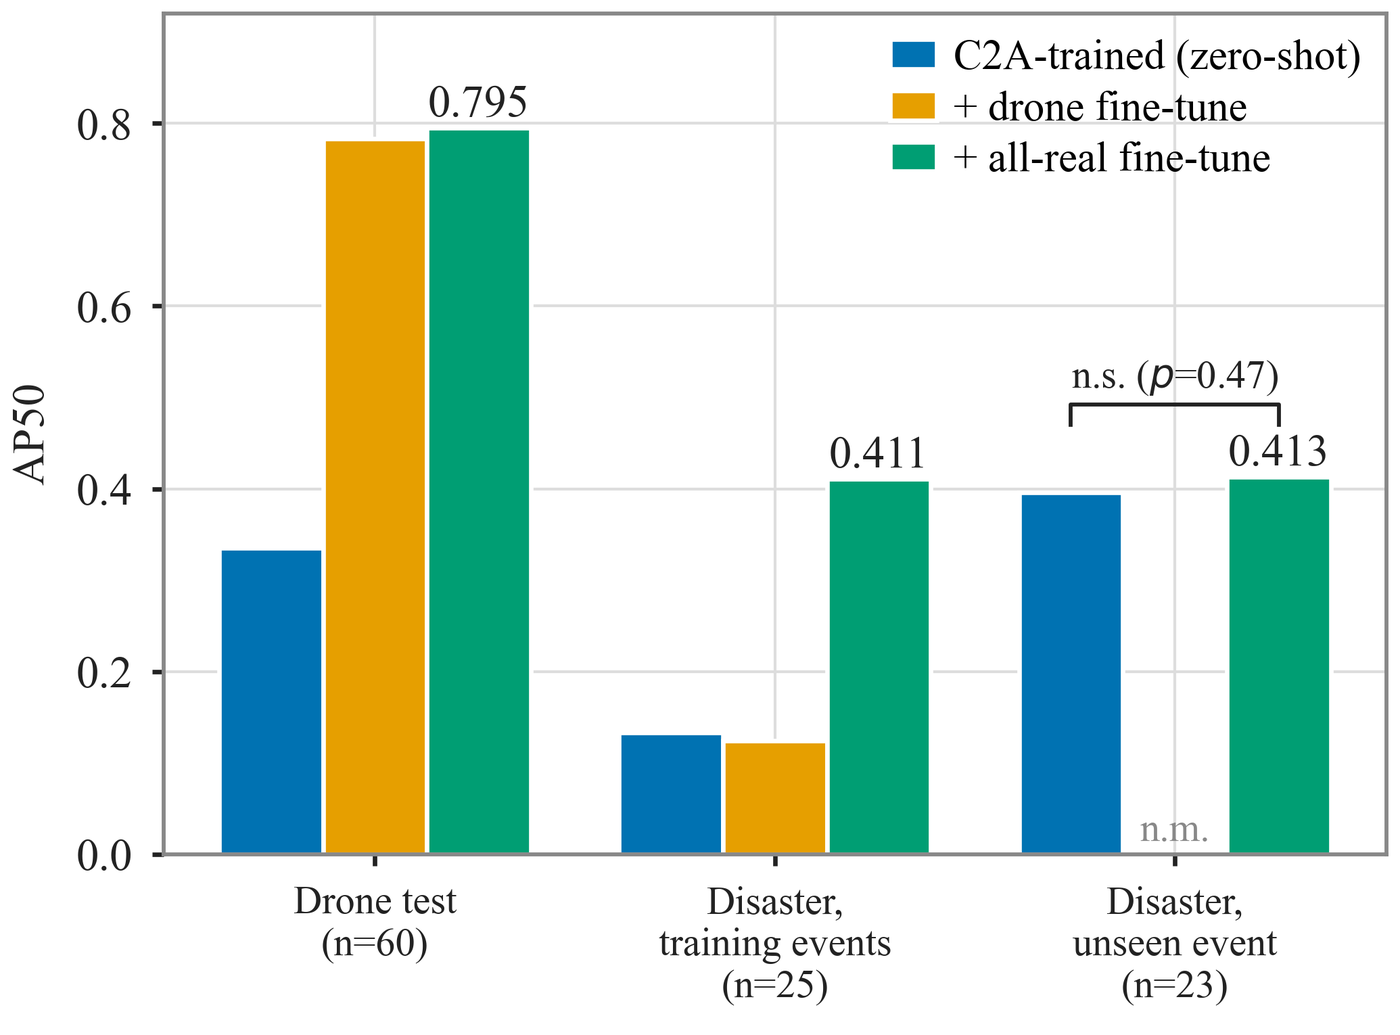
\includegraphics[width=\columnwidth]{figures/fig_adapt_stages_print.png}}
\caption{AP50 of three training stages on the three real evaluation domains.
Drone-only fine-tuning leaves disaster footage untouched (middle bars), so what
helps disaster frames is disaster labels rather than real images in general. On
an event held out from all training (right group) the adapted and base models are
statistically indistinguishable, which bounds the result.}
\label{fig:stages}
\end{figure}

\begin{table}[htbp]
\caption{The Adapted Model on Every Held-Out Set}
\label{tab:multi}
\begin{center}
\small
\begin{tabular}{|l|c|c|c|c|}
\hline
\textbf{Evaluation set} & \textbf{Images} & \textbf{AP50} & \textbf{F2} & \textbf{Rec.} \\
\hline
C2A, scene-disjoint test & 2{,}040 & 0.837 & 0.824 & 0.821 \\
\hline
Drone test & 60 & 0.795 & 0.771 & 0.837 \\
\hline
Campus & 25 & 0.689 & 0.666 & 0.718 \\
\hline
Disaster, training events & 25 & 0.411 & 0.472 & 0.451 \\
\hline
Disaster, unseen event & 23 & 0.413 & 0.451 & 0.374 \\
\hline
\end{tabular}
\end{center}
\end{table}

Three boundaries belong in the record. First, the adaptation is specific to the
footage it saw: on the held-out event the adapted model scores 0.413 against the
base model's 0.396, a difference of 1.7 points whose bootstrap interval spans
zero ($p = 0.47$), while precision at the operating threshold falls by 13.1
points. Sixty frames from two events adapt the model to those events, not to
disasters in general. Second, absolute performance on real disaster imagery
remains modest. At the operating threshold the adapted model finds 482 of 1{,}070
people, and roughly half of its detections are false alarms, which suits
operator-reviewed triage rather than autonomous decisions. Third, people below 8
px in real disaster frames are not recovered at all, across all 54 such
instances, so the size regime this architecture targets on synthetic data is
still open on real data.

\section{Conclusion}
MSA-YOLO enhances YOLO11m for tiny aerial humans with two changes, and the value
of each was measured rather than assumed. The stride-4 detection scale is what
matters, lifting AP50 to 0.853 and sub-8-pixel recall to 0.757, while the
attention substitution pays for itself by removing parameters. A state-space
neck, tested identically, earned nothing for 2.4 million parameters and 2.8 times
the latency. Beyond the network, a tiny-aware assignment blend added 2.08 points
of sub-8-pixel recall at no inference cost, positive in all three seeds tested,
which suggests that for targets this small the training-time assignment of
supervision deserves as much attention as the architecture. On real footage the
same detector fell to 0.335 AP50 on drone video and 0.133 on disaster frames
until 248 labeled real frames raised those to 0.795 and 0.411 at almost no cost
to the benchmark. The remaining gap is concentrated below 8 px on real imagery
and across unseen disaster events, and both point at data collection rather than
architecture as the next step.

\bibliographystyle{IEEEtran}
\bibliography{references}

\end{document}
